\documentclass[../main.tex]{subfiles}

\begin{document}
    \subsection{Lab 2}
    Während dem Durchlauf des Experimentes des Lab 2, werden diverse Daten physikalische Vorgängen
    gesammelt. Diese Daten umfassen Ort und Geschwindigkeit, sowie kinetische und potentielle Energie.
    Dabei wird zwischen dem elastischen sowie inelastischen Zusammenstoss unterschieden.
    \subsubsection{Elastisch}
    Nachfolgend werden alle Daten als Funktion der Zeit zu dem elastischen Zusammenstoss in der
    Abbildung~\ref{fig:GeschwindigkeitAlsFunktionDerZeit} bis Abbildung~\ref{fig:OrtAlsFunktionDerZeit}
    aufgegliedert.

    \begin{figure}[H]
        \begin{center}
            \centerline{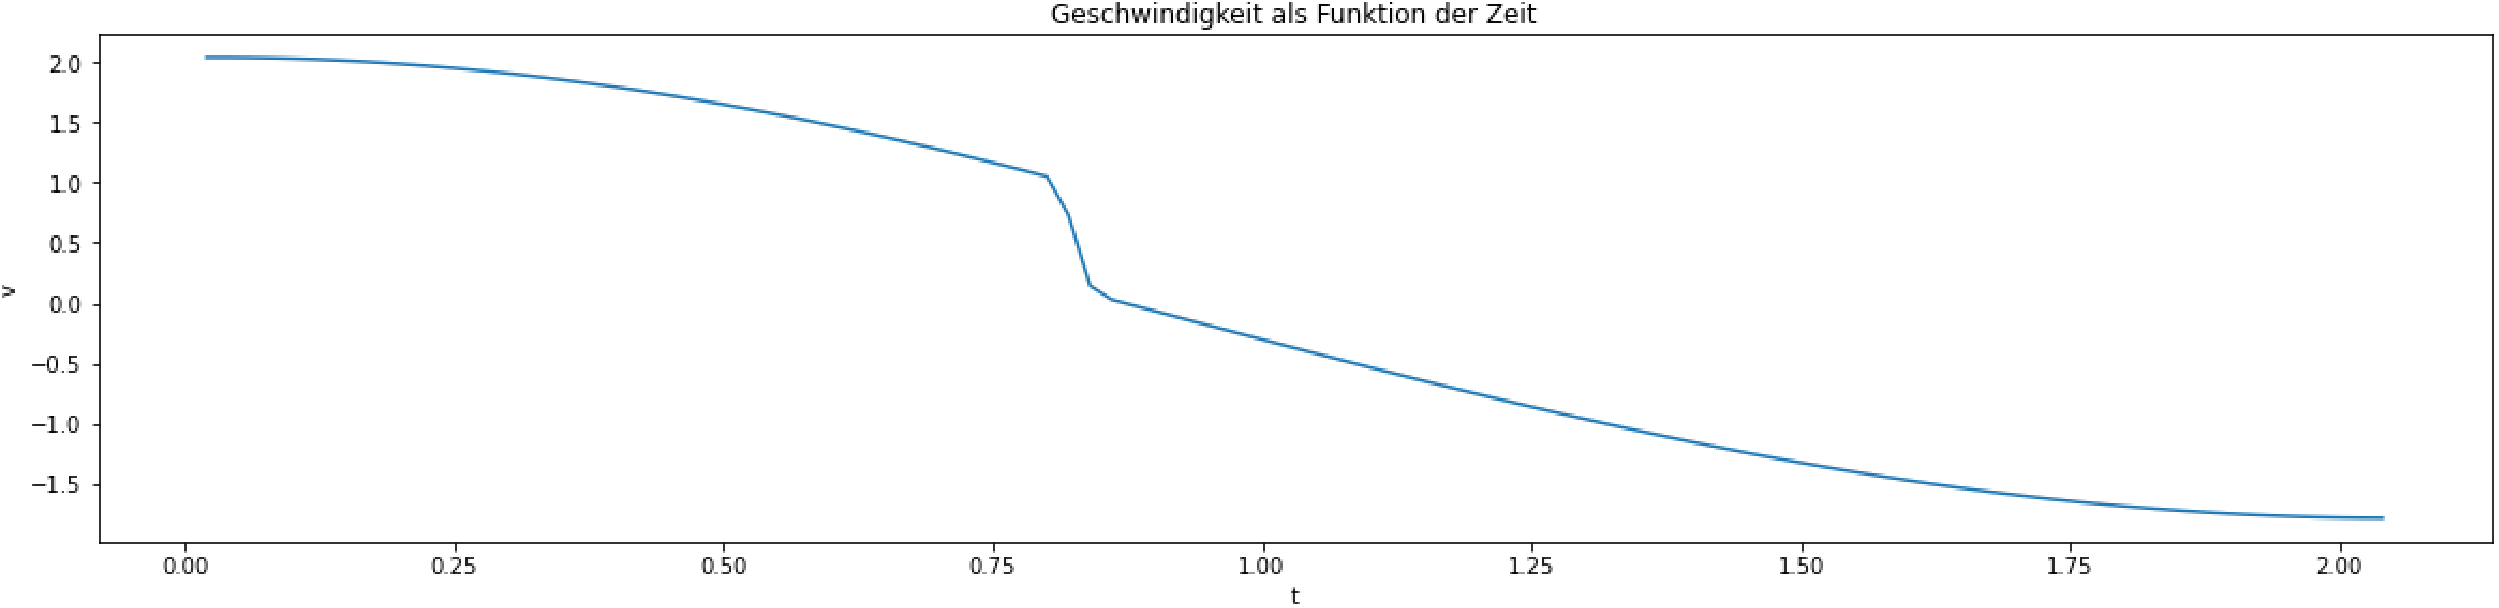
\includegraphics[width=105mm]{./images/Elastisch/GeschwindigkeitAlsFunktionDerZeit}}
            \caption{Geschwindigkeit als Funktion der Zeit}
            \label{fig:GeschwindigkeitAlsFunktionDerZeit}
        \end{center}
    \end{figure}

    \begin{figure}[H]
        \begin{center}
            \centerline{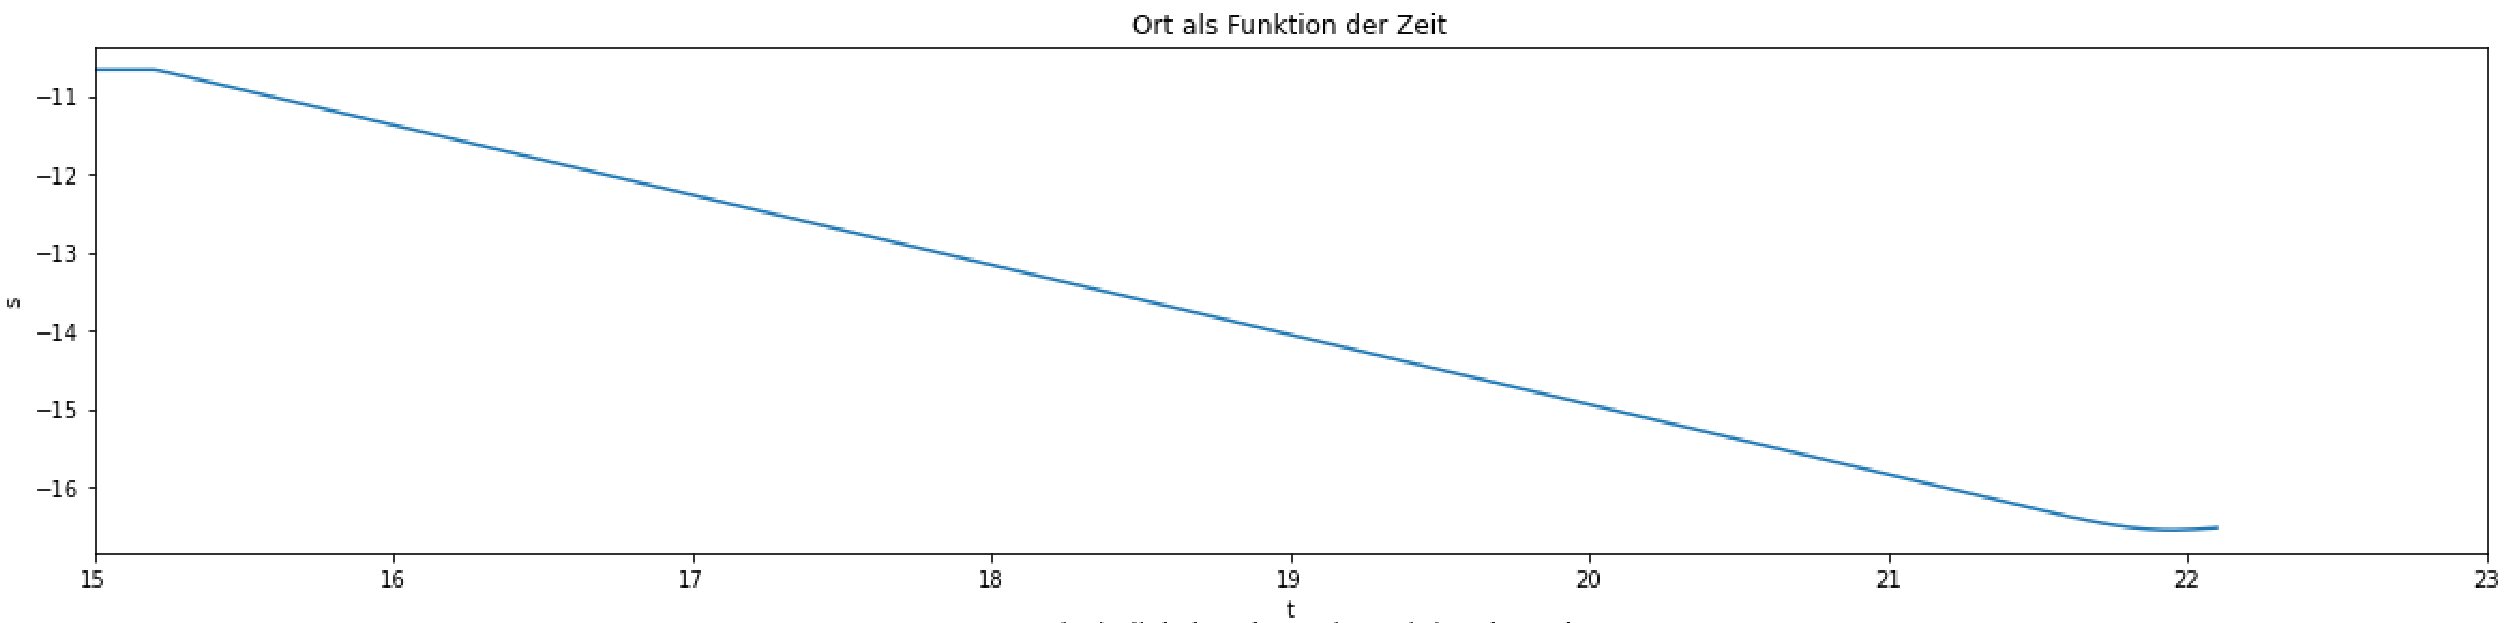
\includegraphics[width=105mm]{./images/Elastisch/OrtAlsFunktionDerZeit}}
            \caption{Ort als Funktion der Zeit}
            \label{fig:OrtAlsFunktionDerZeit}
        \end{center}
    \end{figure}

    \newpage
    \subsubsection{Inelastisch}
    Nachfolgend werden alle Daten als Funktion der Zeit zu dem inelastischen Zusammenstoss in der
    Abbildung~\ref{fig:gesamtImpuls} bis Abbildung~\ref{fig:Endgeschwindigkeit}
    aufgegliedert.
    \newline
    \newline
    In Abbildung~\ref{fig:gesamtImpuls} ist deutlich zu erkennen, wie Romeo
    während der Beschleunigungsphase in den ersten Sekunden an Impuls gewinnt. 
    Nach fünf Sekunden Gleitphase stösst Romeo auf die Feder, wodurch er abgebremst
    wird und Impuls verliert, bis er schliesslich bei null ankommt. Der Impuls wird
    jedoch in der gespannten Feder gespeichert und beim Entspannen der Feder wieder
    auf den Würfel übertragen. Dadurch hat der Würfel nach der Beschleunigungsphase 
    wieder den gleichen Impuls wie zuvor. Der Gesamtimpuls bleibt auch nach der Kollision
    mit Julia gleich, da das Diagramm den Impuls beider Würfel berücksichtigt.
    \begin{figure}[H]
        \begin{center}
            \centerline{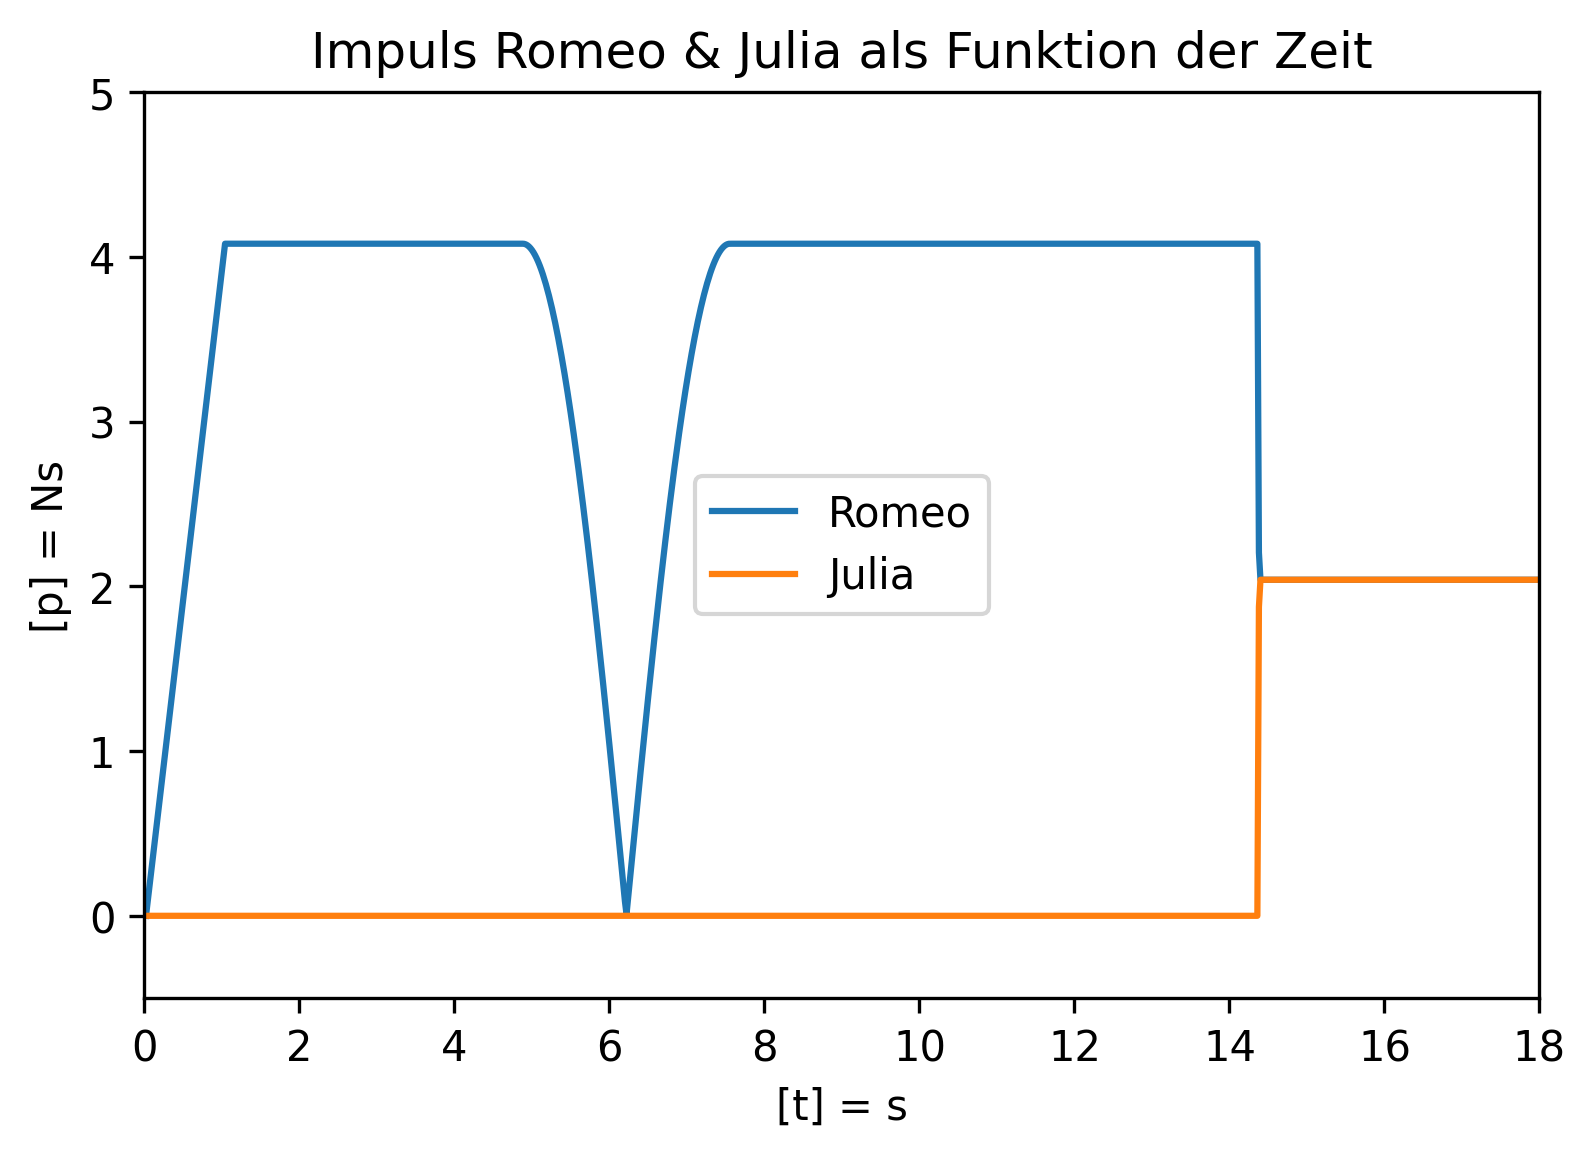
\includegraphics[width=105mm]{./images/Inelastisch/ImpulsRomeoJulia}}
            \caption{Impuls Romeo \& Julia als Funktion der Zeit}
            \label{fig:ImpulsRomeoJulia}
        \end{center}
    \end{figure}

    \begin{figure}[H]
        \begin{center}
            \centerline{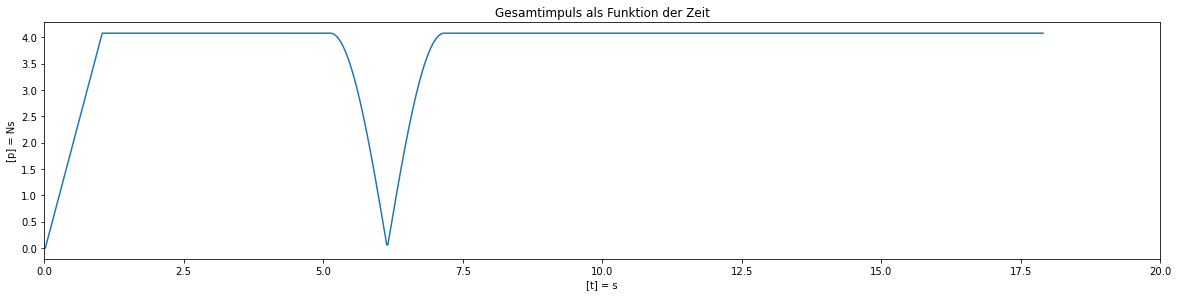
\includegraphics[width=105mm]{./images/Inelastisch/GesamtImpluls}}
            \caption{GesamtImpluls als Funktion der Zeit}
            \label{fig:gesamtImpuls}
        \end{center}
    \end{figure}

    Im Ort-Zeit Diagramm in der Abbildung~\ref{fig:OrtRomeoJuliaAlsFunktionDerZeit} ist ersichtlich, dass Romeo bis Sekunde 5 sich bewegt und danach auf die Feder auftritt, also der elastische Stoss stattfindet. Romeo bewegt sich dann gleichmässig  in die entgegengesetze Richtung und nach 14 Sekunde ist zu sehen wie beide Würfel zusammen sich bewegen. Dort 

    \begin{figure}[H]
        \begin{center}
            \centerline{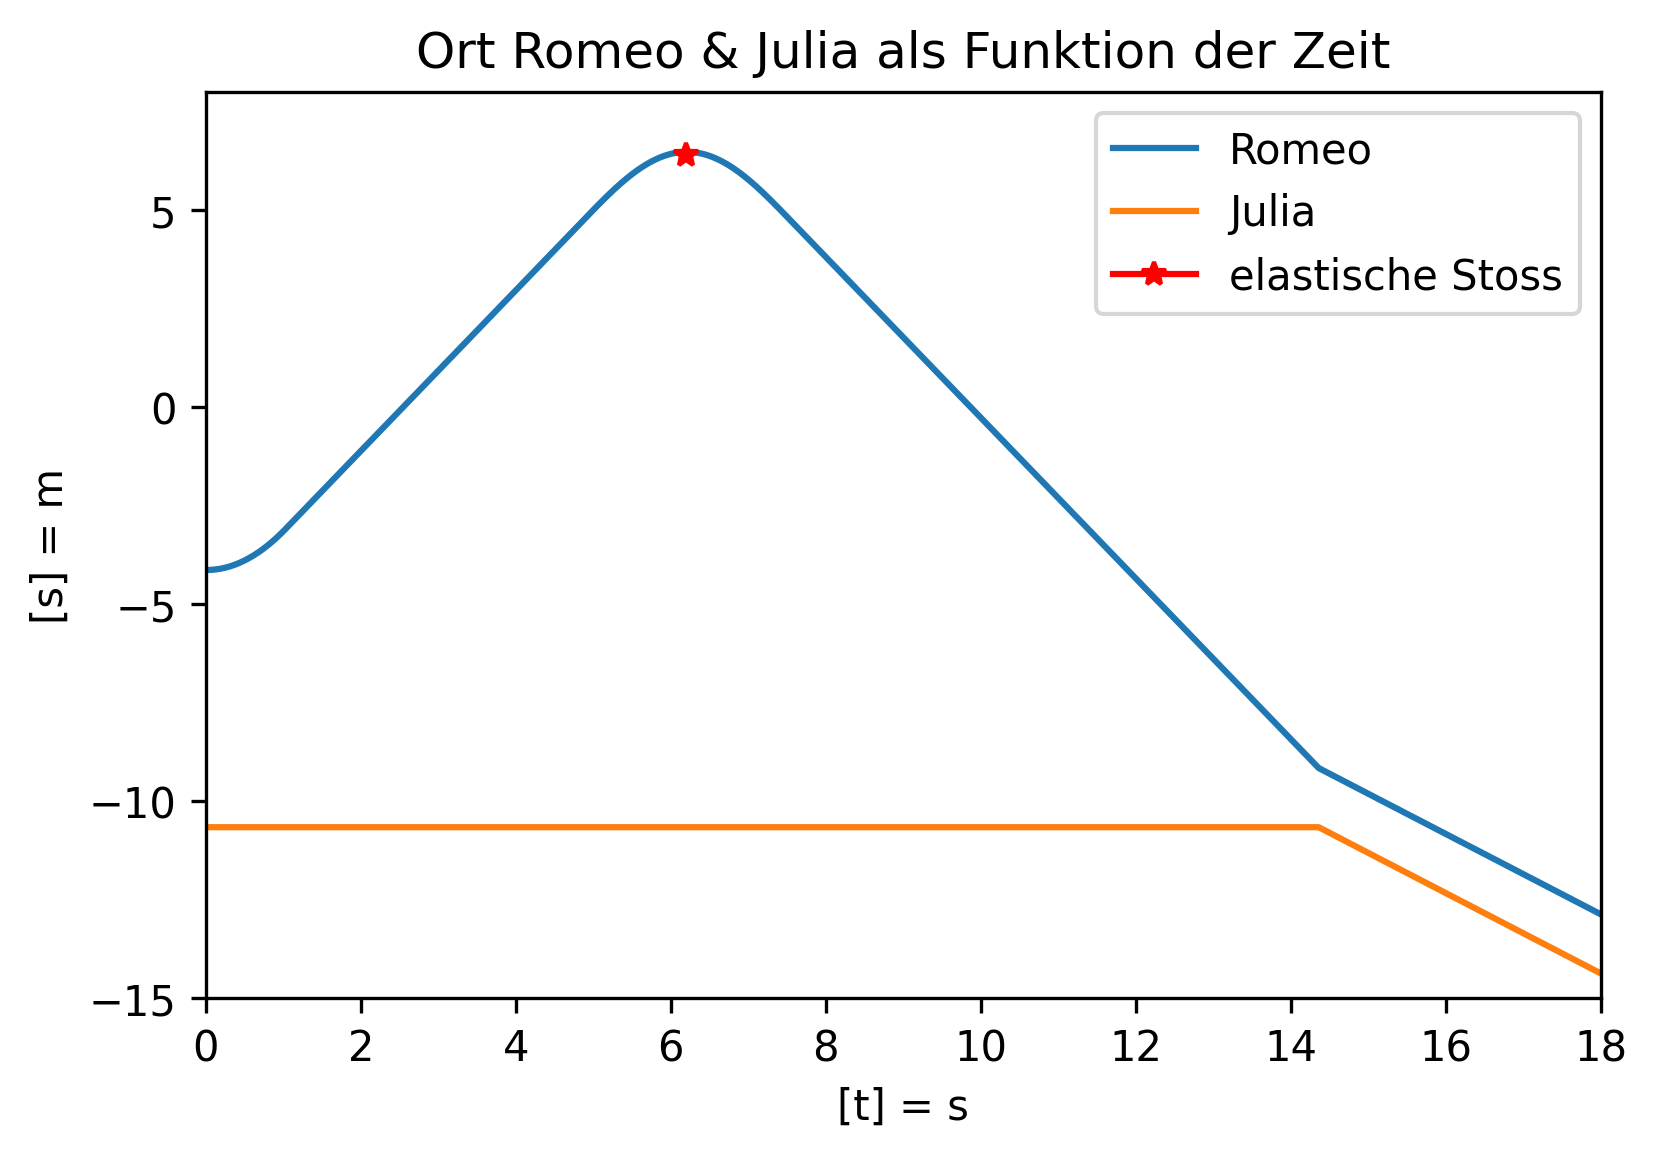
\includegraphics[width=105mm]{./images/Inelastisch/OrtRomeoJuliaAlsFunktionDerZeit}}
            \caption{Ort Romeo \& Julia als Funktion der Zeit}
            \label{fig:OrtRomeoJuliaAlsFunktionDerZeit}
        \end{center}
    \end{figure}

    Gemäss Berechnung erreicht Romeo nach einer Sekunde die maximale Geschwindigkeit von 2 m/s und bewegt sich weiter mit dieser Geschwindigkeit bis es auf die Feder trifft bei circa 5 Sekunden. Dann verändert sich wegen den Rüchstoss die Richtung der Geschwindigkeit. Beim inelastischen Stoss trifft Romeo auf Julia auf und die Geschwindigkeit teilt sich auf die beiden auf. 
    \begin{figure}[H]
        \begin{center}
            \centerline{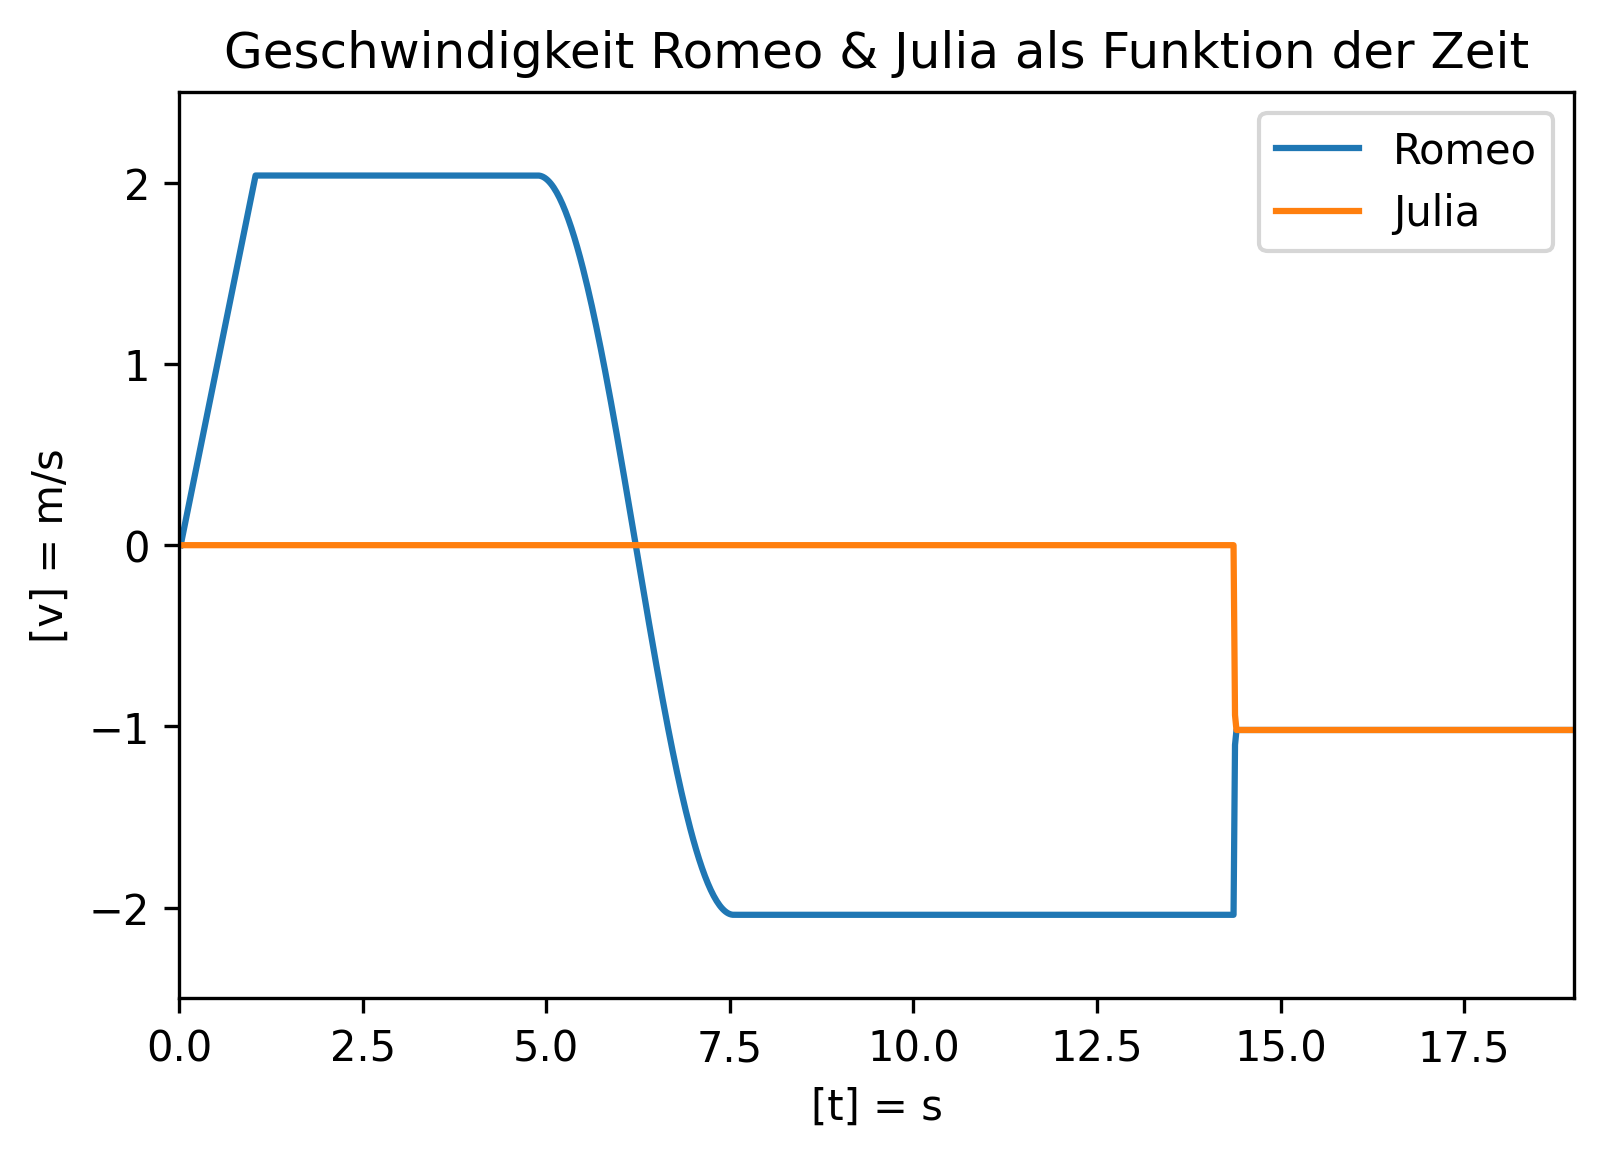
\includegraphics[width=105mm]{./images/Inelastisch/GeschwindigkeitRomeoJulia}}
            \caption{Geschwindigkeit Romeo \& Julia als Funktion der Zeit}
            \label{fig:GeschwindigkeitRomeoJulia}
        \end{center}
    \end{figure}

    \begin{figure}[H]
        \begin{center}
            \centerline{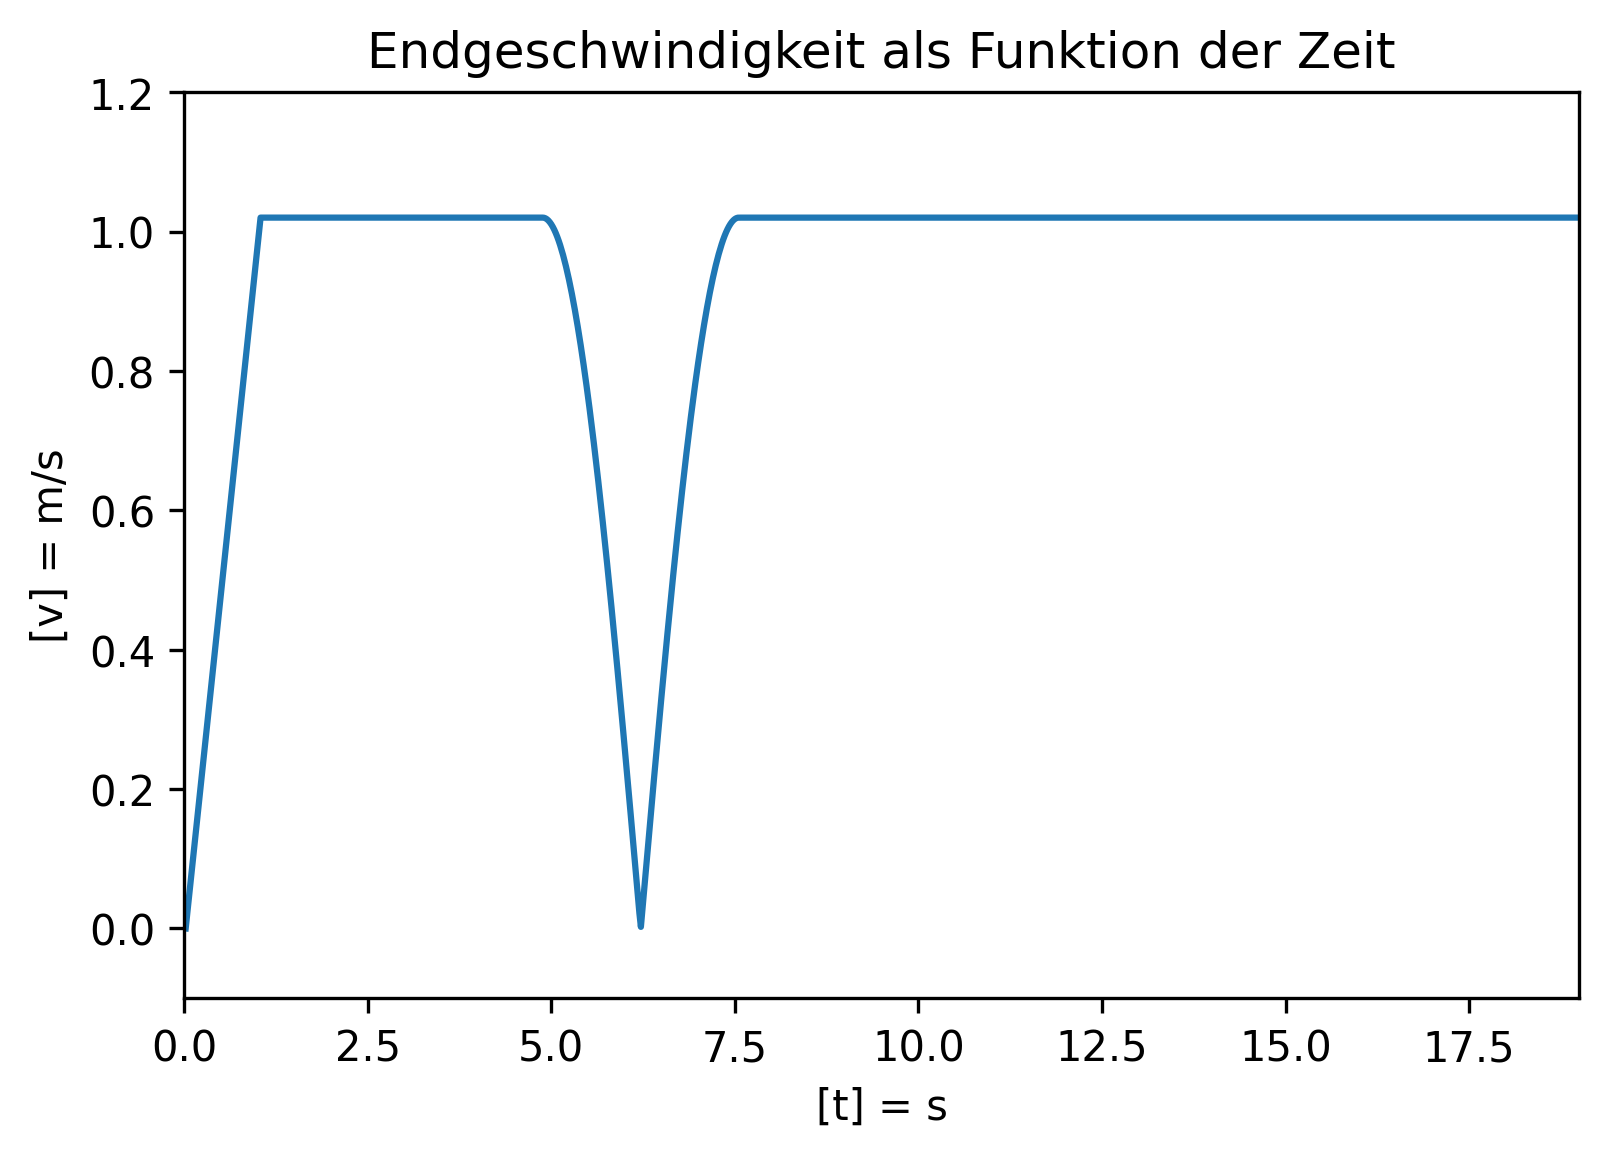
\includegraphics[width=105mm]{./images/Inelastisch/Endgeschwindigkeit}}
            \caption{Endgeschwindigkeit als Funktion der Zeit}
            \label{fig:Endgeschwindigkeit}
        \end{center}
    \end{figure}



\end{document}